\documentclass[9pt]{article}

\usepackage{ifpdf}
\ifpdf 
    \usepackage[pdftex]{graphicx}   % to include graphics
    \pdfcompresslevel=9 
    \usepackage[pdftex,     % sets up hyperref to use pdftex driver
            plainpages=false,   % allows page i and 1 to exist in the same document
            breaklinks=true,    % link texts can be broken at the end of line
            colorlinks=true,
            pdftitle=Knowledge-based generalization of metabolic models
            pdfauthor=Zhukova et al.
           ]{hyperref} 
    \usepackage{thumbpdf}

\else 
    \usepackage{graphicx}       % to include graphics
    \usepackage{hyperref}       % to simplify the use of \href
\fi 
    \usepackage{setspace}
    \usepackage[authoryear]{natbib}
    \usepackage{fullpage}


\title{Knowledge-based generalization of metabolic models}

\author{Anna~Zhukova\thanks{corresponding author - anna.zhukova@inria.fr}\\ Inria Bordeaux Sud-Ouest/University of Bordeaux/CNRS UMR 5800\\
joint project-team Magnome\\
351, cours de la Lib\'{e}ration F-33405 Talence cedex, France
        \and David~James~Sherman\thanks{david.sherman@inria.fr}, \\ Inria Bordeaux Sud-Ouest/University of Bordeaux/CNRS UMR 5800\\
        joint project-team Magnome\\
351, cours de la Lib\'{e}ration F-33405 Talence cedex, France}

\date{}
\setstretch{1}
\newcounter{fig}
\newcounter{pbm}
\newcounter{lm}
\newcounter{def}
\newcounter{rm}

\begin{document}
\maketitle
\newpage

\begin{abstract}
{\bf Background:} Genome-scale metabolic model reconstruction is a complicated process including (semi-)automatic inference of reactions participating in the organism's metabolism, followed by many iterations of network analysis and improvement. More advanced automatic model inference and analysis tools are being developed, but they may still miss some reactions or add erroneous ones. That is why the human expert's analysis of the model plays an important role at all the iterations of the reconstruction process. However, the size of the genome-scale models (i.e. thousands of reactions) makes it hard for a human to analyse them.

{\bf Results:} To aid a human expert in metabolic model analysis we have developed a method for knowledge-based generalization that provides a higher-level view of a metabolic model, by masking inessential details while preserving its essential structure. The method groups biochemical species in the model into semantically equivalent classes and generalizes them into their common parent in the ChEBI ontology. The reactions between the same generalized species are factored together into generalized reactions.

{\bf Conclusions:} We have applied our method to a genome-scale yeast metabolic model and shown that it improves understanding by helping to identify the peculiarities and potential errors.      
\end{abstract}

\paragraph*{Keywords:}metabolic modelling; generalization; genome-scale reconstruction.

\newpage
\section*{Introduction}
Genome-scale metabolic models for new organisms include thousands of reactions. In most cases these reactions are automatically inferred by methods that combine databases of reactions and pathways with genomic information and existing models for similar organisms~\citep{Swainston2011}. Genomic data for the new organism is compared to the data of the reference organism, to find genomic evidence such as the presence of catalysing enzymes for the reactions conserved in the new organism. Starting from the inference of a draft model, the model refinement process includes several iterations of model analysis, error detection, and improvement~\citep{Thiele2010}. The models produced at each iteration are intended for computer simulation, and so describe all the reactions thought to participate in the organism's metabolism. Although automatic model inference tools and genome comparison methods are becoming more advanced, they still may leave gaps in the model or add erroneous reactions. Thus, model evaluation by human experts remains important at all the iteration steps. However, because of their completeness, genome-scale models are too detailed and complicated to be easily understood by a~human. The abundance of reactions in the model may hide errors.


Much of the complexity of the graph comes from similar reactions that operate on slightly different substrates. For example, in the peroxisome compartment of \emph{Yarrowia lypolitica} model (\emph{MODEL1111190000}~\citep{Loira12}) 6 \emph{acetyl-CoA oxidase} reactions are present, transforming \emph{fatty acyls-CoA} different in their carbon chain length (\emph{decanoyl-CoA}, \emph{lauroyl-CoA}, etc.) into corresponding \emph{unsaturated fatty acyls-CoA}. There are also several similar reactions for other steps of \emph{beta-oxidation of fatty acyls} pathway~\citep{Metzler01}. But it is not these details, common for many models, that are interesting for a curator, but the differences from the common pattern, such as missing steps or alternative reactions that use different types of substrates. For a computer simulation though all these details are needed.


%For example, if in a genome-scale model of an yeast \textit{Yarrowia lypolitica} (\emph{MODEL1111190000}~\citep{Loira12}) the enzyme \textit{EC 2.3.1.16} were missing, a whole group of \textit{Acyl-CoA:acetyl-CoA C-acyltransferase} reactions participating in the \textit{Beta-oxidation of fatty acids} pathway~\citep{Metzler01} would be eliminated: one for each of the six \textit{3-oxoacyl-CoA} species presented in the model. However, the absence of these six reactions would be hidden by the other 59 reactions in the constitutive peroxisome of \textit{Yarrowia lypolitica}, and a human expert may have difficulty noticing the error.

To aid human understanding of genome-scale models, while keeping the details needed for a computer simulation, a 3-level \emph{zoomable} approach can be used, with two abstract levels intended for a human expert and the last one for the computer. 

The most abstract level represents compartmentalization of the model, and focusses on such questions as: Are all the compartments present? Are they well connected by transport reactions? 

The second level shows the modules inside of each of the compartments. The questions to be addressed on this level include: Are all the essential processes present? Is the process' structure correct? Is there any organism-specific adaptation of the structure?

The most detailed level is intended for computer simulation and represents the inner structure of each of the modules with all the species, reactions and their kinetics, stoichiometry and constraints.

In this study we focus on the second level of abstraction, that represents the modules inside compartments. A fair amount of work has been done on identifying reusable modules. These approaches can be divided into two groups: \emph{series} and \emph{parallel}. The \emph{series} approaches operate with chains of reactions, and generalize them as a series, thus hiding the structure of the network. An example of a \emph{series} approach is representing the network as a set of metabolic pathways (KEGG~\citep{Kanehisa12}, MetaCyC~\citep{Caspi2012}), that can be further divided, for example, into reaction modules (conserved sequences of reactions along the metabolic pathways)~\citep{Muto2013}. 

The other type of approaches operates with reactions that are \emph{parallel}, thus keeping the steps and preserving the general view of the network. An example of this approach is grouping reactions based on EC (Enzyme Commission) numbers~\citep{Tohsato2000}. The drawback of this approach is that it is not applicable to networks with no EC number assigned or reactions with no catalysing enzymes identified. 
We developed another \emph{parallel}-reaction method for knowledge-based generalization of metabolic models, that does not depend on enzyme information. It provides a~higher-level view of a~model while keeping its essential structure and omitting the details. 


\newtheorem{eq00}[def]{Definition}
\begin{eq00}
The \emph{model generalization} process groups chemical species present in the model into equivalence classes, and merges them into a generalized chemical species. Reactions that involve same generalized chemical species are then factored together into a generalized reaction. 
\end{eq00}

By applying the model generalization process, we can build a simplified model that focusses on the high level relationships. The simplified model can be further divided into pathways. 

\newpage
\section*{Mathematical basis}

\subsection*{Basic definitions}

We represent a \emph{metabolic model $M$} as a pair of two sets: a set $S$ of biochemical species, and a set $R$ of reactions between them: 

\[ \begin{array}{ccll}
\mbox{$M$} & \mbox{$=$} & \mbox{$\langle S, R \rangle$} & \mbox{- model,} \\
\mbox{$S$} & \mbox{$=$} & \mbox{$\{s_1, \ldots, s_n\}$} &  \mbox{- species set,} \\
\mbox{$R$} & \mbox{$=$} & \mbox{$\{r_1, \ldots, r_m\}$} &  \mbox{- reaction set.} 
\end{array} \]

We represent each \emph{reaction $r \in R$} as a pair of species sets: its reactants and products. A chemical reaction may be represented by a balanced chemical equation, showing the formulae of the reactants and products, and the changes that take place~\citep{Clugston2000}. This definition leads to the restriction~(1) that all the species participating in the reaction must be different.

\[ \begin{array}{llr}
\mbox{$r = $} & \mbox{$\langle\{s^{(rs)}_1, \ldots, s^{(rs)}_k\},\{s^{(ps)}_1, \ldots, s^{(ps)}_l\}\rangle
\in R \subset \langle 2^S \times 2^S \rangle$}, &\\
& \mbox{where } \mbox{$s^{(rs)}_1 \neq \ldots \neq s^{(rs)}_k \neq s^{(ps)}_1 \neq \ldots \neq s^{(ps)}_l$}  & (1)
\end{array} \]

To perform the model generalization, we define an \emph{equivalence operation $\sim$} on the species set, and group species into equivalence classes: $[s]^{\sim} = \{\tilde{s} \in S | \tilde{s} \sim s\}$.

Species equivalence imposes reaction equivalence: two reactions are equivalent if their corresponding reactant and product species are pairwise equivalent.
\[ \begin{array}{l}
\mbox{$\forall r, \tilde{r} \in R $} \begin{array}{c}
	\mbox{$r = \langle\{s^{(rs)}_1, \ldots, s^{(rs)}_k\},\{s^{(ps)}_1, \ldots, s^{(ps)}_l\}\rangle,$}\\
	\mbox{$\tilde{r} = \langle\{\tilde{s}^{(rs)}_1, \ldots, \tilde{s}^{(rs)}_{\tilde{k}}\},\{\tilde{s}^{(ps)}_1, \ldots, \tilde{s}^{(ps)}_{\tilde{l}}\}\rangle$}
\end{array}\\ 
\mbox{$r \sim \tilde{r} \iff \; \land$} \begin{array}{l}
	\mbox{$k = \tilde{k}, l = \tilde{l}$}, \\
	\mbox{$\forall i\; 0\leq{i}\leq{k} \; \exists{!} \tilde{i}\; 0\leq \tilde{i}\leq \tilde{k}:\; s^{(rs)}_i \sim \tilde{s}^{(rs)}_{\tilde{i}}$}, \\
	\mbox{$\forall j\;0\leq j\leq l\;\exists{!} \tilde{j}\;0\leq \tilde{j}\leq\tilde{l}:\;s^{(ps)}_j \sim \tilde{s}^{(ps)}_{\tilde{j}}$}.
\end{array}	 
\end{array} \]

Equivalent reactions are factored together into a generalized reaction that operates with generalized species (i.e. species equivalence classes): 
$[r]^{\sim} = \langle\{[s^{(rs)}_1]^{\sim}, \ldots, [s^{(rs)}_k]^{\sim}\}, \{[s^{(ps)}_1]^{\sim}, \ldots, [s^{(ps)}_l]^{\sim}\}\rangle$.

In order to keep the number of distinct species participating in a reaction, the restriction~(1'), analogous to the restriction~(1), must be satisfied:
\[ \begin{array}{lr}
\mbox{$[s^{(rs)}_1]^{\sim} \neq \ldots \neq [s^{(rs)}_k]^{\sim} \neq [s^{(ps)}_1]^{\sim} \neq \ldots \neq [s^{(ps)}_l]^{\sim}$} & (1')
\end{array} \]

In order to avoid creation of paths in the generalized model that are not based on the evidence from the initial model, we introduce the restriction~(2): Species that do not participate in any pair of equivalent reactions and do not have any common equivalent species must not be grouped together.
\[ \begin{array}{clr}
\mbox{$\forall s, \tilde{s} \in S\; s \sim \tilde{s} \;\Rightarrow\;\lor$} & 
\begin{array}{l}
	\mbox{$\exists r \sim \tilde{r} \in R: s \in reactants(r) \land \tilde{s} \in reactants(\tilde{r})$} \\
	\mbox{$\exists r \sim \tilde{r} \in R: s \in products(r) \land \tilde{s} \in products(\tilde{r})$} \\
	\mbox{$ \exists \dot{s} \in S:\; s \tilde{\sim} \dot{s} \land \dot{s} \tilde{\sim} \tilde{s}$}.
\end{array} & (2)
\end{array} \]
Note, that restriction~(2) can be reformulated as maximizing the number of species equivalence classes while keeping the reaction equivalence classes unchanged. 

The \emph{generalized model $M/\sim$} is a pair of generalized species and reaction sets (quotient sets):
\[ \begin{array}{ccll}
\mbox{$M/\sim$} & \mbox{$=$} & \mbox{$\langle S/\sim, R/\sim \rangle$} & \mbox{ - generalized model,} \\
\mbox{$S/\sim$} & \mbox{$=$} & \mbox{$\{[s_1]^{\sim}, \ldots, [s_{\tilde{n}}]^{\sim}\}$} &  \mbox{ - quotient species set,} \\
\mbox{$R/\sim$} & \mbox{$=$} & \mbox{$\{[r_1]^{\sim}, \ldots, [r_{\tilde{m}}]^{\sim}\}$} &  \mbox{ - quotient reaction set.} 
\end{array} \]

The generalized model is a zoom out of the initial model. It provides a higher-level view by including less species and reactions, but more generic ones. For example, \textit{3-oxodecanoyl-CoA}, \textit{3-oxolauroyl-CoA}, and \textit{3-oxohexanoyl-CoA} species of the initial model can be generalized into \textit{oxo-fatty acyl-CoA}. 

Every reaction of the generalized model corresponds to at least one reaction of the initial model having the same topology (number of distinct reactant and product species) and operating with species that can be zoomed out into those participating in the generalized reaction. The appropriate level of abstraction is defined by the initial model as the most general one that satisfies restrictions (1') and (2).

The method and restrictions are described in figure~\ref{fig:mg}.

\begin{figure}[th]
\centering
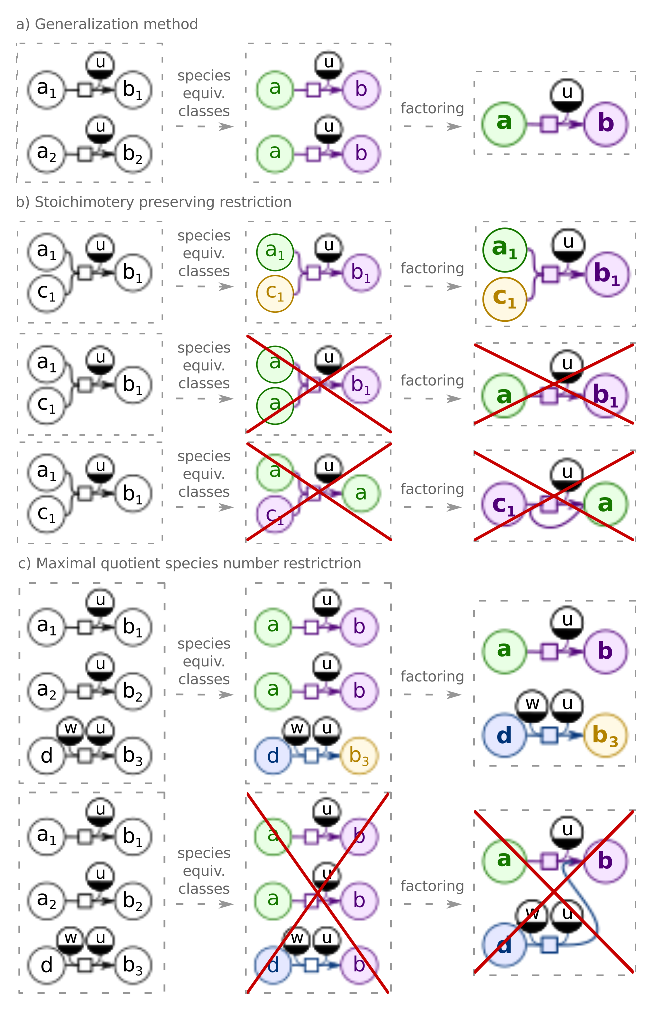
\includegraphics{../pics/Zhukova_Fig_1.eps}
\caption{\textbf{Model generalization method and restrictions.} 
\textbf{a)} \textit{The generalization method} first groups the species into equivalence classes, and then factors them into generalized species. The reaction equivalence classes and factoring are based on the species ones.
\textbf{b)} \textit{The restriction (1').} The top part shows a correct generalization that obeys the restriction. Two bottom parts show generalizations that change the reaction stoichiometry, and thus are not allowed.
\textbf{c)} \textit{The restriction (2).} The top part shows a correct generalization that obeys the restriction. The bottom part violates the restriction as there is no evidence in the model (i.e. no equivalent reaction) of the species $b_3$ belonging to the same equivalence class as $b_1$ and $b_2$.}
\label{fig:mg}
\end{figure}

\subsubsection*{Specific and ubiquitous species}
We say that a \emph{ubiquitous species} is one that participates in many reactions (e.g. more than a threshold), such as \emph{water}, \emph{hydrogen}, \emph{oxygen}, etc. Grouping species increases the number of reactions they participate in, while they are already shared by many reactions and common to most of the models. During visualisation these species are often even duplicated to improve readability~\citep{Rohn2012}. That is why we do not generalize them. In the generalized model each of them forms a trivial equivalence class:
\[ \begin{array}{l}
\mbox{$S^{(ub)} = \{s^{(ub)}_1, \ldots, s^{(ub)}_{\breve{n}}\} \subset S: \forall i\,[s^{(ub)}_i]^{\sim} = \{s^{ub}_i\}$} 
\end{array} \]

\emph{Specific species} are the others, they are divided into non-trivial equivalence classes and generalized accordingly.  

\subsection*{Model generalization problem}
\newtheorem{p0}[pbm]{Problem}
\begin{p0}
Given a metabolic model $M=\langle S, S^{(ub)} \subset S, R \rangle$ that describes $n$ species (including $\breve{n} \leq n$ ubiquitous ones) and $m$ reactions, find an equivalence operation $\sim$ that obeys the restrictions~(1') and (2), and minimizes the number of reaction equivalence classes $\sharp R/\sim$.
\end{p0}

We will solve the model generalization problem~1 in three steps:
\begin{enumerate}
\item Define the most general equivalence operation $\mathring{\sim}$ (having minimal number of species equivalence classes $\sharp{S/\mathring{\sim}}$), that does not take into account the restrictions;
\item Modify the current equivalence operation to satisfy the restriction~(1');
\item Modify the current equivalence operation to satisfy the restriction~(2).
\end{enumerate}

\subsubsection*{Step 1. Equivalence operation $\mathring{\sim}$.}
\newtheorem{eq0}[def]{Definition}\label{equiv0}
\begin{eq0}
Given a model $M=\langle S, S^{(ub)}\subset{S}, R \rangle : \sharp S = n, \sharp S^{(ub)}=\breve{n} \leq n, \sharp R = m$, we define an \emph{equivalence operation $\mathring{\sim}$} on the species set $S$ as forming $\breve{n} + 1$ equivalence classes in the quotient set $S/\mathring{\sim}$: one for each of the ubiquitous species, and one for all the other species:
\[ \begin{array}{cl}
\mbox{$\forall s^{(ub)} \in S^{(ub)}$} & \mbox{$[s^{(ub)}]^{\mathring{\sim}} = \{s^{(ub)}\}$}, \\
\mbox{$\forall s, \tilde{s} \in S\backslash S^{(ub)}$} & \mbox{$[s]^{\mathring{\sim} } = [\tilde{s}]^{\mathring{\sim} } = S \backslash S^{(ub)}$}. 
\end{array} \]

\end{eq0}
\newtheorem{l1}[lm]{Lemma}
\begin{l1}
For any equivalence operation $\sim$ on the model $M=\langle S, S^{(ub)} \subset S, R \rangle$, the corresponding quotient species set $S/\sim$ and quotient reaction set $R/\sim$ are partitions of respectively the quotient species set $S/\mathring{\sim}$ and the quotient reaction set $R/\mathring{\sim} $ induced by $\mathring{\sim}$:
\[ \begin{array}{c}
\mbox{$\forall $ equivalence operation $\sim$ defined on $\langle S, S^{(ub)}, R \rangle$} \\
\begin{array}{cl}
\mbox{$\forall s \in S$} & \mbox{$[s]^{\sim} \subset [s]^{\mathring{\sim}}$} \\
\mbox{$\forall r \in R$} & \mbox{$[r]^{\sim} \subset [r]^{\mathring{\sim}} $}
\end{array}
\end{array} \]

\end{l1}

%\paragraph*{Algorithm 1 - Computation of $\mathring{\sim}$}
\[ \begin{array}{l}
\mbox{\textbf{Algorithm: }Compute$\mathring{\sim}$}\\
\mbox{\textbf{Data: }} \begin{array}{l} \mbox{$M=\langle{S, S^{(ub)}\subset{S}, R}\rangle: \sharp S = n, \sharp S^{(ub)}=\breve{n} \leq n, \sharp R = m$ - metabolic model}\\ \mbox{describing $n$ species,  $\breve{n}$ among them being ubiquitous,  and $m$ reactions.} 
\end{array}\\
\mbox{\textbf{Result: }} \begin{array}{l} \mbox{$\mathring{\sim}$ - equivalence operation described in Lemma~1,}\\  \mbox{$M/{\mathring{\sim}} = \langle S/{\mathring{\sim}}, S^{(ub)}/{\mathring{\sim}} \subset S/{\mathring{\sim}}, R/{\mathring{\sim}} \rangle$ - corresponding generalized model.} \end{array}\\
\mbox{~}\\
\mbox{$S/{\mathring{\sim}} \leftarrow \emptyset;$ // resultant quotient species set $ S/{\mathring{\sim}}\subset 2^S$}\\
\mbox{$S^{(ub)}/{\mathring{\sim}} \leftarrow \emptyset;$ // resultant quotient ubiquitous species set $ S^{(ub)}/{\mathring{\sim}}\subset 2^{S^{(ub)}}$}\\
\mbox{$R/{\mathring{\sim}} \leftarrow \emptyset;$ // resultant quotient reaction set $ R/{\mathring{\sim}}\subset 2^R$}\\
\mbox{$\mathring{\sim} \leftarrow \emptyset;$ // resultant equivalence operation $ {\mathring{\sim}}: S\cup{R} \rightarrow S/{\mathring{\sim}}\cup{R/{\mathring{\sim}}}$}\\
\mbox{~}\\
\mbox{/* Generalize ubiquitous species */}\\
\mbox{\textbf{for }$s^{(ub)} \in S^{(ub)}$\textbf{ do}}\\
\left| \indent\mbox{$[s^{(ub)}]^{\mathring{\sim}} \leftarrow \{s^{(ub)}\};$ // map $s^{(ub)}$ to its equivalence class}\right. \\
\mbox{\textbf{end}}\\
\mbox{$S^{(ub)}/{\mathring{\sim}} \leftarrow \{[s^{(ub)}]^{\mathring{\sim}}|s^{(ub)} \in S^{(ub)}\};$}\\
\mbox{~}\\
\mbox{/* Generalize specific species */}\\
\mbox{\textbf{for }$s \in S \backslash S^{(ub)}$\textbf{ do}}\\
\left| \indent\mbox{$[s]^{\mathring{\sim}}   \leftarrow S \backslash S^{(ub)};$ // map $s$ to its equivalence class}\right. \\
\mbox{\textbf{end}}\\
\mbox{$S/{\mathring{\sim}} \leftarrow {S^{(ub)}/{\mathring{\sim}}}\cup\{S \backslash S^{(ub)}\};$}\\
\mbox{~}\\
\mbox{/* Generalize reactions */}\\
\mbox{// map a reaction to its generalized version that operates with generalized species}\\
\mbox{$gen \leftarrow \lambda{r}.\langle\{[s]^{\mathring{\sim}} | s \in reactants(r)\}, \{[s]^{\mathring{\sim}} | s \in products(r)\}\rangle;$}\\
\mbox{\textbf{for }$r \in R$\textbf{ do}}\\
\left| \indent\mbox{$[r]^{\mathring{\sim}} \leftarrow \{\tilde{r} \in R|gen(\tilde{r})=gen(r)\};$}\right. \\
\mbox{\textbf{end}}\\
\mbox{$R/{\mathring{\sim}} \leftarrow \{[r]^{\mathring{\sim}}|r \in R\};$}\\
\mbox{~}\\
\mbox{\textbf{return }$\mathring{\sim}, \langle S/{\mathring{\sim}}, S^{(ub)}/{\mathring{\sim}}, R/{\mathring{\sim}} \rangle$}
\end{array} \]
The Compute$\mathring{\sim}$ algorithm forms the equivalence classes for ubiquitous and then specific species as in Definition~2 and then computes the generalized reactions.

\subsection*{Step 2. Stoichiometry preserving property obedience}
\newtheorem{p2}[pbm]{Problem}
\begin{p2}
Given an equivalence operation $\sim$ defined on a metabolic model $M=\langle S, S^{(ub)}\subset{S}, R \rangle$ find an equivalence operation $\breve{\sim}$ that obeys the restriction~(1') and induces a quotient species set $S/\breve{\sim}$ of minimal size $\sharp S/\breve{\sim}$, such that $S/\breve{\sim}$ is a partition of the quotient species set $S/{\sim}$ induced by $\sim$, i.e., $\forall s \in S \; [s]^{\breve{\sim}} \subset [s]^{\sim} $. 
\end{p2}
\subsubsection*{Algorithm}
We start with the given equivalence operation $\sim^0 = \sim$, and iteratively improve it, until the stoichiometry preserving property~(1') is obeyed. We denote the equivalence operation obtained at the $i$-th iteration step as $\sim^i$.

At each iteration, if there exists a species equivalence class that violates the stoichiometry preserving property~(1'), i.e.:
\[ \begin{array}{l}
\mbox{$\exists s \neq \tilde{s} \in S, r \in R: s \in species(r) \land \tilde{s} \in species(r) \land  [s]^{{\sim}^i} = [\tilde{s}]^{{\sim}^i}$}, 
\end{array} \]
we partition this species equivalence class $[s]^{{\sim}^i} = [\tilde{s}]^{{\sim}^i}$ into two: $[s]^{{\sim}^{i+1}}  \vee [\tilde{s}]^{{\sim}^{i+1}}  = [s]^{{\sim}^i} = [\tilde{s}]^{{\sim}^i} $ to form a new approximation ${\sim}^{i+1}$ of the equivalence operation. When no species equivalence class violating the restriction~(1') can be found, the current equivalence operation is returned as result.

At each iteration one equivalence species class is partitioned. In the worst case, the equality operation $=$ (each species is equivalent only to itself) will be achieved. As it obeys the restriction~(1'), the process will terminate. \\

%\subsubsection*{Algorithm 2 - Stoichiometry Preserving Property Obedience}
\[ \begin{array}{l}
\mbox{\textbf{Algorithm: }PreserveStoichiometry}\\
\mbox{\textbf{Data: }} \begin{array}{l} \mbox{${\sim}$ - equivalence operation defined on a metabolic model $M=\langle S, S^{(ub)}\subset{S}, R \rangle$,}\\ \mbox{$M/{\sim} = \langle S/{\sim}, S^{(ub)}/{\sim} \subset S/{\sim}, R/{\sim} \rangle$ - corresponding generalized model.} 
\end{array}\\
\mbox{\textbf{Result: }} \begin{array}{l} \mbox{$\breve{\sim}$ - equivalence operation described in Problem~3,}\\  \mbox{$M/\breve{\sim} = \langle S/\breve{\sim}, S^{(ub)}/\breve{\sim} \subset S/\breve{\sim}, R/\breve{\sim} \rangle$ - corresponding generalized model.} \end{array}\\
\mbox{~}\\
\mbox{$S/\breve{\sim} \leftarrow S/\sim;$ // resultant quotient species set $ S/{\breve{\sim}}\subset 2^S$}\\
\mbox{$S^{(ub)}/\breve{\sim} \leftarrow S^{(ub)}/\sim;$ // resultant quotient ubiquitous species set $ S^{(ub)}/{\breve{\sim}}\subset 2^{S^{(ub)}}$}\\
\mbox{$R/\breve{\sim} \leftarrow \emptyset;$ // resultant quotient reaction set $ R/{\breve{\sim}}\subset 2^R$}\\
\mbox{$\breve{\sim} \leftarrow \sim;$ // resultant equivalence operation $ {\breve{\sim}}: S\cup{R} \rightarrow S/{\breve{\sim}}\cup{R/{\breve{\sim}}}$}\\
\mbox{~}\\

\mbox{/* Partition quotient species that do not obey the stoichiometry preserving property~(1') */}\\
\mbox{\textbf{for }$S^{(gen)} \in \{\tilde{S}^{(gen)}\in S/\breve{\sim}| \exists s \neq \tilde{s} \in \tilde{S}^{(gen)}, r \in R:  s \in species(r) \land \tilde{s} \in species(r)\}$\textbf{ do}}\\
\left| \indent \begin{array}{l}
\mbox{$\Pi = Partition(S^{(gen)});$}\\
\mbox{} \\
\mbox{// Update $S/\breve{\sim}$} \\
\mbox{$S/\breve{\sim} \leftarrow S/\breve{\sim}\backslash\{S^{(gen)}\};$} \\
\mbox{$S/\breve{\sim} \leftarrow S/\breve{\sim}\cup\Pi;$} \\
\mbox{} \\
\mbox{// Update $\breve{\sim}$} \\
\mbox{\textbf{for }$\tilde{S}^{(gen)} \in \Pi$\textbf{ do}} \\
\left| \indent \begin{array}{l}
\mbox{\textbf{for }$s \in \tilde{S}^{(gen)}$\textbf{ do}}\\
\left| \indent\mbox{$[s]^{\breve{\sim}} \leftarrow \tilde{S}^{(gen)};$}\right. \\
\mbox{\textbf{end}}
\end{array}\right. \\
\mbox{\textbf{end}}
\end{array}\right. \\
\mbox{\textbf{end}}\\
\mbox{~}\\
\mbox{/* Generalize reactions */}\\

\mbox{// map a reaction to its generalized version that operates with generalized species}\\
\mbox{$gen \leftarrow \lambda{r}.\langle\{[s]^{\breve{\sim}} | s \in reactants(r)\}, \{[s]^{\breve{\sim}} | s \in products(r)\}\rangle;$}\\

\mbox{\textbf{for }$r \in R$\textbf{ do}}\\
\left| \indent \mbox{$[r]^{\breve{\sim}} \leftarrow \{\tilde{r} \in R|gen(\tilde{r})=gen(r)\};$}\right. \\
\mbox{\textbf{end}}\\
\mbox{$R/{\breve{\sim}} \leftarrow \{\breve{\sim}(r)|r \in R\};$}\\
\mbox{~}\\
\mbox{\textbf{return }$\breve{\sim}, \langle S/\breve{\sim}, S^{(ub)}/\breve{\sim}, R/\breve{\sim} \rangle$}
\end{array} \]

\subsubsection*{Species equivalence class partition}

%\subsubsection*{Clique partition}
%\newtheorem{scg}[def]{Definition}
%\begin{scg}
%For a given a set of species and a set of reactions between them, we define a \emph{species compatibility graph} as a simple undirected graph with vertices representing the species, and edges linking those of the species that do not participate in the same reaction (i.e., putting them into the same equivalence class does not violate the stoichiometry preserving property~(1')).
%\end{scg}
%Note, that any set of species that can be put into the same equivalence class without violating the stoichiometry preserving property~(1'), forms a clique  in the species compatibility graph, i.e. a complete subgraph: for every pair of its vertices there exists an edge linking them. Thus, the problem of partition the species equivalence class into minimum number of classes, such that all of them obey the stoichiometry preserving property~(1') is a clique partition problem.
%\newtheorem{clp}[pbm]{Problem}
%\begin{clp}[Clique partition]
%Find the smallest number of cliques in a graph such that every vertex in the graph is represented in exactly one clique.
%\end{clp}
%\newtheorem{rem0}[rm]{Remark}
%\begin{rem0}
%Clique partition problem is known to be \textit{NP}-complete~\citep{Bhasker1991}. 
%\end{rem0}


%In a species compatibility graph, there are usually a few edges missing
In a species equivalence class that violates the restriction~(1') there are usually only a few conflicts present, and multiple solutions of the partition problem exist. 

\subsubsection*{Species ontology}
In order to make the choice of the species equivalence classes biologically meaningful, we use an ontology that describes hierarchical \textit{is\_a} relationships (i.e. more specific - more general) between biochemical species. %This ontology can be viewed as a directed acyclic graph, with nodes representing terms describing species, and edges representing hierarchical relationships between them. A term $T$ is an ancestor of a term $t$ if and only if there exists a path from $t$ to $T$. 

\newtheorem{mt}[def]{Definition}
\begin{mt}
A term $t$ is a \emph{model term} if it corresponds to a specific species in the metabolic model. 
\end{mt}
We assume that no two model terms are connected by a descendant-ancestor relationship in the ontology (Otherwise, we mark the ancestor term ubiquitous): \\
\[ \begin{array}{c}
\mbox{$\forall t, T \in terms \; (\exists\, species(t), species(T) \in S \land t \in descendants(T) \Rightarrow t = T)$.}
\end{array} \]

We iteratively remove all the leaf terms that are not model terms from the ontology, so that all the model terms become leaves, and all the leaves become model terms. 

For each species equivalence class that needs to be partitioned, we first find the least common ancestor $T$ of the ontological terms corresponding to its species. If the ontology allows for multiple inheritance, and there are several such least common ancestors, we pick the first one. Then we look among the $T$-th descendant terms for those that are compatible (to avoid multiple inheritance).

\newtheorem{comp}[def]{Definition}
\begin{comp}
Terms $ t_1, \ldots, t_k$ are \emph{compatible} if and only if their descendant model terms do not intersect:
$ t_1, \ldots, t_k$ are compatible $\iff \forall i \neq j \in \{1, \ldots, k\} \; descendants(t_i) \cap descendants(t_k) \cap leaves(T) = \emptyset$.
\end{comp}

\newtheorem{pp}[pbm]{Problem}
\begin{pp}
Given a term $T$, find a compatible term set among its descendants, such that it has minimal size, covers all the $T$-th descendant leaf terms, and satisfies the stoichiometry preserving property~(1''):
\[ \begin{array}{ll}
\mbox{$?\; t_1, \ldots, t_k \in descendants(T):\; \land $} & \begin{array}{lr}
	\mbox{$k = k_{min}$},&\\
	\mbox{$t_1, \ldots, t_k$ are compatible,} & \\
	\mbox{$leaves(T) \subset descendants(t_1) \cup \ldots \cup descendants(t_k)$},  & \\
	\begin{array}{l}
	\mbox{$\forall i \neq j \in \{1, \ldots, k\}\;\forall t \in leaves(t_i), \tilde{t} \in leaves(t_j)$} \\
	\indent \mbox{$\forall r \in R \; \{species(t), species(\tilde{t})\} \not \subset species(r)$}.
	\end{array} & (1'')
\end{array}
\end{array} \]

\end{pp}
To do so, we first exclude all the terms that violate the stoichiometry preserving property~(1''). We thus obtain an exact set cover problem.
% We say that a subset $S$ covers its own elements.

\newtheorem{setc}[pbm]{Problem}
\begin{setc}[Set cover]
Given a set $X$ and a collection of its finite subsets $\Psi$, such that $\bigcup_{S \in \Psi} S = X$, find a minimum-size subset $\Pi \subset \Psi$ whose members cover all of $X$: $\bigcup_{S \in \Pi} S = \bigcup_{S \in \Psi} S = X$.
\end{setc}
\newtheorem{rem}[rm]{Remark}
\begin{rem}
 Set cover is \textit{NP}-complete~\citep{karp72}.
\end{rem}

\newtheorem{esetc}[pbm]{Problem}
\begin{esetc}[Exact set cover]
As in \emph{Set cover} problem, except that here the sets used in the cover are not allowed to intersect. 
\end{esetc}
\newtheorem{rem1}[rm]{Remark}
\begin{rem1}
Exact cover is \textit{NP}-complete~\citep{Goldreich2008}.
\end{rem1}

\subsubsection*{Exact set cover applied to ontological terms}
Each ontological term $t$ defines a set $S(t)$ of its descendant leaf terms (including $t$ if it is a leaf). The instance consists of a set $X$ of the model terms of interest, and a collection $\Psi$ of all sets defined by their common ancestor $T$, its descendant terms, and their relative complements with respect to $X$: $\forall S \in \Psi \; X\backslash S \in \Psi$, excluding all the sets that violate the stoichiometry preserving property~(1''). We look for a minimum-size exact cover of $X$. 

Note, that in this case an exact cover always exists, e.g. the one formed by all the leaf terms.

\subsubsection*{Choice of the ontology}
We assume that any term that violates property~(1'') is removed from the ontology. Note, that the term $T$ is also removed.

If the ontology has no multiple inheritance, i.e. $\forall S, \tilde{S} \in \Psi \; S \cap \tilde{S} \neq \emptyset \Rightarrow S \subseteq \tilde{S} \lor \tilde{S} \subseteq S$, the problem becomes trivial: The set of the root terms forms the solution. The size of the solution though depends on the characteristics of the ontology, e.g. for a completely flat ontology (i.e., with no relationships) the solution consists of singleton equivalence classes.

If the multiple inheritance is allowed, any $\Psi \subseteq 2^X$ becomes possible, and the problem becomes \textit{NP}-complete. 

We will use the ChEBI ontology~\citep{deMatos10} of chemical compounds, as it is \textit{de facto} a standard for species annotation in metabolic models. ChEBI consists of three main branches: \textit{chemical entity}, \textit{role}, and \textit{subatomic particle}. The \textit{chemical entity} branch describes terms useful for annotation of biochemical species in a metabolic model. %As of ChEBI version 101, this branch contains 37693 terms, among which 29888 are leaves. ChEBI has multiple inheritance with average number of parents 1.4 per term. Average number of siblings is also 1.4 per term. Maximal depth in the \textit{chemical entity} branch is 28, while the average one is 11.

The level of details in the ChEBI hierarchy is not uniform: some sub-branches are more developed than others, which makes equally precise terms to be placed unequally deep in the hierarchical tree. For example, both \textit{hydrogen peroxide (CHEBI:16240)} and \textit{decanoyl-CoA (CHEBI:28493)} terms describe precise chemical molecules; but \textit{hydrogen peroxide} is only 5 terms away from the \textit{chemical entity} in the ChEBI hierarchy, while \textit{decanoyl-CoA} is 11 terms away. 

Besides that, different types of classification are combined together in the hierarchical tree, leading to multiple inheritance. For example, in the \textit{fatty-acid (CHEBI:35366)} sub-branch, several classification types are present, including:
\begin{itemize}
\item classification based on the length of the carbon chain:
\begin{itemize}
\item \textit{short-chain fatty acid (CHEBI:26666)}: 2-4 carbons;
\item \textit{medium-chain fatty acid (CHEBI:59554)}: 6-12 carbons;
\item etc.
%\item \textit{long-chain fatty acid (CHEBI:15904)}: 14-22 carbons;
%\item \textit{very long-chain fatty acid (CHEBI:27283)}: 24 -26 carbons;
\end{itemize}
\item classification based on the presence of double bonds in the carbon chain:
\begin{itemize}
\item \textit{saturated fatty acid (CHEBI:26607)}: no double bonds;
\item \textit{unsaturated fatty acid (CHEBI:27208)}: one or more double bonds;
\end{itemize}
\item classification based on substituent groups:
\begin{itemize}
\item \textit{hydroxy fatty acid (CHEBI:24654)}: one or more hydroxy substituents;
\item \textit{oxo fatty acid (CHEBI:59644)}: at least one aldehydic or ketonic group;
\item etc.
\end{itemize}
\end{itemize}

Moreover, using only hierarchical relationships in the ChEBI ontology is not always enough. Examples show, that similar reactions can happen to the acid and the base in a conjugate acid-base pair. A conjugate acid-base pair is two species, one an acid and one a base, that differ from each other through the loss or gain of a proton~\citep{stoker2012general}. For instance, in the Rhea database of chemical reactions~\citep{Alcantara2012}, the \textit{acyl-CoA oxidase (RHEA:28354)} reaction: $\textit{decanoyl-CoA} + \textit{FAD} + \textit{H+} \rightarrow \textit{trans-dec-2-enoyl-CoA} + $\textit{FADH$_2$} is found for both \textit{decanoyl-CoA~(CHEBI:28493)} and its conjugate base \textit{decanoyl-CoA(4-)~(CHEBI:61430)}. But hierarchically these species are very far from each other in the ChEBI ontology: Their least common ancestor is \textit{molecular entity (CHEBI:23367)}, a direct descendant of the root \textit{chemical entity}. To establish a conjugate acid-base pair correspondence in the ChEBI ontology not the hierarchical (\textit{is\_a}) but special \textit{is\_conjugate\_base\_of}/\textit{is\_conjugate\_acid\_of} relationships are used. To maximize the chances of a conjugate acid-base pair being in the same quotient species set, we generalize the hierarchical relationship.

\newtheorem{dirgent}[def]{Definition}
\begin{dirgent}
Term $t$ is a \emph{generalized direct descendant/ancestor} of a term $T$ if and only if $t$ or a conjugate base or acid of $t$ is a direct descendant/ancestor of $T$ or of a conjugate base or acid of $T$.
\end{dirgent} 

\newtheorem{gent}[def]{Definition}
\begin{gent}
Term $t$ is a \emph{generalized descendant/ancestor} of a term $T$ if and only if $t$ is a generalized direct descendant/ancestor of $T$ or of any generalized descendant/ancestor of $T$.
\end{gent} 

We extend $\Psi$ so that it has closure under the operation of relative complement: $\forall S,\tilde{S} \in \Psi \; S\backslash\tilde{S} \in \Psi$. This allows for solving the set cover problem instead of the exact cover one:  As $\Psi$ is closed under the operation of complement intersection, we can obtain an exact set cover $\tilde{C}$ from any set cover $C = \{S_1, S_2, \ldots, S_m\}$ by replacing its elements with their relative complements with the previous elements of $C$: $\tilde{C} = \{S_1, S_2 \backslash S_1, \ldots, S_m \backslash \bigcup^{m - 1}_{i = 1}{S_i}\}$.

To approximate the solution of the set cover problem, we use a greedy algorithm.

\subsubsection*{Greedy Algorithm}
Among the available subset candidates $S_i \in \Psi$ pick the one of the largest size and add it to the resulting set cover $\Pi$. Repeat this operation until all elements of $X$ are covered. \\

%\subsubsection*{Algorithm 3 - Greedy Set Cover}
\[ \begin{array}{l}
\mbox{\textbf{Algorithm: }GreedySetCover}\\
\mbox{\textbf{Data: }}\begin{array}{l}\mbox{$X$ - set of interest,}\\ \mbox{$\Psi \subseteq 2^X$ - set of subsets of $X$}\end{array}\\
\mbox{\textbf{Result: }$\Pi \subseteq \Psi$ - set cover of $X$}\\
\mbox{~}\\
\mbox{$\Pi \leftarrow \emptyset;$ // resultant cover}\\
\mbox{~}\\
\mbox{\textbf{while }$X \neq \emptyset$\textbf{ do}}\\
\left| \indent \begin{array}{l}
\mbox{// select $S \in \Psi$ that covers maximum elements of $X$} \\
\mbox{$S^{(max)} \leftarrow max(\Psi, criterion=\lambda{S}.\sharp{(S\cap{X}}));$} \\
\mbox{~}\\
\mbox{$\Psi \leftarrow \Psi\backslash\{S^{(max)}\};$}\\
\mbox{$X \leftarrow X\backslash{S^{(max)}};$} \\
\mbox{$\Pi \leftarrow \Pi\cup\{S^{(max)}\};$} 
\end{array}\right.\\
\mbox{\textbf{end}}\\
\mbox{~}\\
\mbox{\textbf{return }$\Pi$}
\end{array} \]
Greedy set cover is a polynomial time approximation algorithm that achieves an approximation ratio of $H(\sharp X)$, where $H(n)$ is the $n$-th harmonic number: $H(n) = \sum^n_{i = 1}\frac{1}{i} \leq \ln{n} + 1$~\citep{Chvatal1979}. It is the best-possible polynomial time approximation algorithm for set cover, under plausible complexity assumptions~\citep{Feige1998}. 

\subsection*{Step 3. Species equivalence class number maximization}
\newtheorem{p1}[pbm]{Problem}
\begin{p1}
Given an equivalence operation $\sim$ defined on a metabolic model $M=\langle S, S^{(ub)}\subset{S}, R \rangle$, find an equivalence operation $\tilde{\sim}$ that obeys restriction~(2) and does not change the reaction equivalence classes: $R/\sim = R/\tilde{\sim}$. 
\end{p1}
\subsubsection*{Algorithm}
To satisfy the restriction~(2) we associate each species $s$ in the initial model with a pair of reaction equivalence classes sets in the quotient reaction set $R/{\sim}$: induced by reactions where it participates as a reactant or product. \\
$s \rightarrow \langle R^{(rs)}_s = \{[r^{(rs)}_1]^{\sim}, \ldots, [r^{(rs)}_o]^{\sim}\}, R^{(ps)}_s = \{[r^{(ps)}_1]^{\sim}, \ldots, [r^{(ps)}_t]^{\sim}\}\rangle$.

\newtheorem{eq1}[def]{Definition}\label{equiv1}
\begin{eq1}
Given an equivalence operation $\sim$ defined on a metabolic model $M=\langle S, S^{(ub)}\subset{S}, R \rangle$, we define an \emph{equivalence operation $\tilde{\sim}$} as forming a separate species equivalence class for each of the ubiquitous species, and putting $\sim$-equivalent specific species that intersect in their product or reactant reaction classes in the same equivalence class:
\[ \begin{array}{rll}
\mbox{$\forall s^{(ub)} \in S^{(ub)}, s \in S \;\; s^{(ub)} \tilde{\sim} s$} & \mbox{$\iff$} & \mbox{$s^{(ub)} = s$}, \\
\mbox{$\forall s, \tilde{s} \in S \backslash S^{(ub)} \;\; s \tilde{\sim} \tilde{s}$} & \mbox{$\iff \;\land$} & 
	\begin{array}{l}
		\mbox{$s \sim \tilde{s}$} \\
		\mbox{$(R^{(rs)}_s \cap R^{(rs)}_{\tilde{s}} \neq \emptyset)\;\lor\;$} 
		\mbox{$(R^{(ps)}_s \cap R^{(ps)}_{\tilde{s}} \neq \emptyset)\;\lor\;$}
		\mbox{$(\exists \dot{s} \in S:\; s \tilde{\sim} \dot{s} \land \dot{s} \tilde{\sim} \tilde{s})$}.
	\end{array}
\end{array} \]
\end{eq1}

Any further partition of the quotient species set would imply the partition of the quotient reaction set. Hence the number of species equivalence classes is maximal for the current number of reaction equivalence classes, and the restriction (2) is satisfied.

%\subsubsection*{Algorithm 4 - Maximization of the Number of Species Equivalence Classes}
\[ \begin{array}{l}
\mbox{\textbf{Algorithm: }Maximize}\\
\mbox{\textbf{Data: }} \begin{array}{l} \mbox{${\sim}$ - equivalence operation defined on a metabolic model $M=\langle S, S^{(ub)}\subset{S}, R \rangle$,}\\ \mbox{$M/{\sim} = \langle S/{\sim}, S^{(ub)}/{\sim} \subset S/{\sim}, R/{\sim} \rangle$ - corresponding generalized model.} 
\end{array}\\
\mbox{\textbf{Result: }} \begin{array}{l} \mbox{$\tilde{\sim}$ - equivalence operation described in Problem~2,}\\  \mbox{$M/\tilde{\sim} = \langle S/\tilde{\sim}, S^{(ub)}/\tilde{\sim} \subset S/\tilde{\sim}, R/\tilde{\sim} \rangle$ - corresponding generalized model.} \end{array}\\
\mbox{~}\\
\mbox{$S/\tilde{\sim} \leftarrow \emptyset;$ // resultant quotient species set $ S/{\tilde{\sim}}\subset 2^S$}\\
\mbox{$S^{(ub)}/\tilde{\sim} \leftarrow S^{(ub)}/\sim;$ // resultant quotient ubiquitous species set $ S^{(ub)}/{\tilde{\sim}}\subset 2^{S^{(ub)}}$}\\
\mbox{$R/\tilde{\sim} \leftarrow R/\sim;$ // resultant quotient reaction set $ R/{\tilde{\sim}}\subset 2^R$}\\
\mbox{$\tilde{\sim} \leftarrow \sim;$ // resultant equivalence operation $ {\tilde{\sim}}: S\cup{R} \rightarrow S/{\tilde{\sim}}\cup{R/{\tilde{\sim}}}$}\\
\mbox{~}\\
\mbox{/* Update specific species generalization */}\\
\mbox{~}\\
\mbox{// Map a species to a set of its $\sim$-equivalent species}\\
\mbox{// that participate in $\sim$-equivalent reactions}\\
\mbox{$r\_sim \leftarrow \lambda{s}.\{\tilde{s}\sim{s}|\exists r,\tilde{r}\in{R}: s\in reactants(r) \land \tilde{s}\in reactants(\tilde{r}) \land r \sim \tilde{r}\};$}\\
\mbox{$p\_sim \leftarrow \lambda{s}.\{\tilde{s}\sim{s}|\exists r,\tilde{r}\in{R}: s\in products(r) \land \tilde{s}\in products(\tilde{r}) \land r \sim \tilde{r}\};$}\\
\mbox{$sim \leftarrow \lambda{s}.r\_sim(s)\cup p\_sim(s);$}\\
\mbox{~}\\
\mbox{$S/\tilde{\sim} \leftarrow S^{(ub)}/\tilde{\sim} \cup \{sim(s)|s \in S\backslash S^{(ub)}\};$}\\
\mbox{~}\\
\mbox{// Merge all quotient species sets that intersect}\\
\mbox{\textbf{while }$\exists S^{(gen)} \neq \tilde{S}^{(gen)} \in S/\tilde{\sim}: S^{(gen)} \cap \tilde{S}^{(gen)} \neq \emptyset$\textbf{ do}}\\
\left| \indent\mbox{$S/\tilde{\sim} \leftarrow (S/\tilde{\sim}\backslash{\{S^{(gen)}, \tilde{S}^{(gen)}\}})\cup\{S^{(gen)}\cup \tilde{S}^{(gen)}\};$}\right. \\
\mbox{\textbf{end}}\\
\mbox{~}\\
\mbox{// Update $\tilde{\sim}$}\\
\mbox{\textbf{for }$S^{(gen)}\in{S/\tilde{\sim}}$\textbf{ do}}\\
\left| \indent \begin{array}{l}
\mbox{\textbf{for }$s \in S^{(gen)}$\textbf{ do}}\\
\left| \indent\mbox{$[s]^{\tilde{\sim}} \leftarrow S^{(gen)};$ // map $s$ to its equivalence class}\right. \\
\mbox{\textbf{end}}
\end{array}\right. \\
\mbox{\textbf{end}}\\
\mbox{~}\\
\mbox{\textbf{return }$\tilde{\sim}, \langle S/\tilde{\sim}, S^{(ub)}/\tilde{\sim}, R/\tilde{\sim} \rangle$}
\end{array} \]

%\subsection*{Complete Algorithm}
%As the most complex step of model generalization is the species partition, we precede it with the species equivalence class number maximisation step, in order to minimize the size of each species quotient class to be partitioned. We start with the equivalence operation $\mathring{\sim}$ described in Lemma~1, maximize the species equivalence class number for $\mathring{\sim}$, then obey the stoichiometry preserving property using the ChEBI ontology and greedy set cover algorithm, and finally maximize the species equivalence class number again.\\

\subsection*{Complete algorithm}
\[ \begin{array}{l}
\mbox{\textbf{Algorithm: }Compute${\sim}$}\\
\mbox{\textbf{Data: }}\begin{array}{l}\mbox{$M=\langle{S, S^{(ub)}\subset{S}, R}\rangle: \sharp S = n, \sharp S^{(ub)}=\breve{n} \leq n, \sharp R = m$ - metabolic model}\\ \mbox{describing $n$ species,  $\breve{n}$ among them being ubiquitous,  and $m$ reactions.}\end{array}\\
\mbox{\textbf{Result: }}\begin{array}{l}\mbox{$\sim$ - approximation of the equivalence operation described in Problem~0,}\\ \mbox{$M/\sim = \langle S/\sim, S^{(ub)}/\sim \subset S/\sim, R/\sim \rangle$ - corresponding generalized model.}\end{array}\\
\mbox{~}\\
\mbox{$\mathring{\sim}, M/\mathring{\sim} \leftarrow Compute\mathring{\sim}(M);$} \\
%\mbox{$\tilde{\sim}, M/\tilde{\sim} \leftarrow Maximize(\mathring{\sim}, M/{\mathring{\sim}});$} \\
\mbox{$\breve{\sim}, M/\breve{\sim} \leftarrow PreserveStoichiometry(\mathring{\sim}, M/{\mathring{\sim}});$} \\
\mbox{$\sim, M/\sim \leftarrow Maximize(\breve{\sim}, M/\breve{\sim});$} \\
\mbox{~}\\
\mbox{\textbf{return }$\sim, M/\sim = \langle S/\sim, S^{(ub)}/\sim, R/\sim \rangle$}
\end{array} \]

\newpage
\section*{Applications}
We have applied our method to the genome-scale metabolic network of the yeast \textit{Yarrowia lipolytica} (\emph{MODEL1111190000} \citep{Loira12}). The generalized model is attached as additional files~1, 2. The generalization has created 100 non-trivial quotient species and 217 non-trivial quotient reactions, and reduced  the total number of species from 1847 to 1072 and of reactions from 2002 to 893. %Figures representing compartments before and after generalization are attached as additional files. 

The generalization method shows the best performance if the model is well-annotated with ChEBI. The species lacking ChEBI annotations are forced to form trivial quotient species in the generalized model as there is no evidence of their biochemical similarity with any other species in ChEBI.  For 430 species in the \textit{Y.~lipolytica} model no appropriate ChEBI annotation was found, thus they could not be grouped with other species. 

\emph{Peroxisome} is an example of a well-annotated compartment in the \textit{Y.~lipolytica} model: only two species have no ChEBI annotations: \emph{YLR043C disulphide} and \emph{TRX1}. The generalization process reduced the number of reactions in peroxisome from 65 to 27. Figures~\ref{fig:bf} and \ref{fig:yali} represent the peroxisome before and after the generalization and were produced using Tulip graph visualisation tool~\citep{Auber04}.

The model before the grouping of equivalent reactions and species into generalized ones is shown on figure~\ref{fig:bf}: different colors correspond to different equivalence classes. The same color code is used in figure~\ref{fig:yali} representing the generalized model that operates with quotient species and reactions. For example, the violet \textit{unsaturated FA-CoA} node is a quotient of 8 species: \textit{hexadec-2-enoyl-CoA}, \textit{oleoyl-CoA}, \textit{tetradecenoyl-CoA}, \textit{trans-dec-2-enoyl-CoA}, \textit{trans-dodec-2-enoyl-CoA}, \textit{trans-hexacos-2-enoyl-CoA}, \textit{trans-octadec-2-enoyl-CoA}, and \textit{trans-tetradec-2-enoyl-CoA} (coloured violet in figure~\ref{fig:bf}). In a similar manner, the light-green \textit{acCoA oxidase} quotient reaction, that converts \textit{fatty acyl-CoA} (yellow) into \textit{unsaturated FA-CoA} (violet), generalizes 6 corresponding light-green reactions of the initial model (figure~\ref{fig:bf}).

The generalized model describes \textit{$\beta$-oxidation of fatty acids} pathway~\citep{Metzler01} happening inside \textit{Y.~lypolitica} peroxisome in a generic way: as a transformation of \textit{fatty acyl-CoA} (yellow) into \textit{unsaturated FA-CoA} (violet), then into \textit{hydroxy FA-CoA} (green), \textit{3-oxo FA-CoA} (magenta), and back to \textit{fatty acyl-CoA} (with a shorter carbon chain); while the initial model describes the same process in more details, specifying those reactions for each of the \textit{fatty acyl-CoA} species present in the organisms' cell (e.g. \textit{decanoyl-CoA}, \textit{dodecanoyl-CoA}, etc.). That is why the \textit{beta-oxidation} chain of the reactions in the initial model, transforming step-by-step the \emph{fatty-acyl-CoA} with the longest carbon chain into the one with the shortest chain, in the generalized model appears as a cycle (generalizing all the \textit{fatty-acyls-CoA} into one species, regardless the chain-length).
  
The more precise model is needed for simulation, while the more general one is clearer to a human, and reveals the main properties of the model. For example, the generalized model highlights the fact that there is a particularity concerning \textit{C24:0-CoA (tetracosanoyl-CoA)} (red, inside the cycle in figure~\ref{fig:yali}): There exists a "short-cut" reaction, producing it directly from another \textit{fatty acyl-CoA} (yellow), avoiding the usual four-reaction beta-oxidation chain, used for other \textit{fatty acyls-CoA}.

Another application of model generalization is metabolic model comparison. The generalization brings the models to the same level of abstraction and highlights the differences such as gaps. Examples can be found in~\citep{Zhukova}.


%We have applied our method to three metabolic models that describe the \textit{$\beta$-oxidation of fatty acids} pathway: a genome-scale metabolic model of the yeast \textit{Yarrowia lipolytica} (\emph{MODEL1111190000}), and two path2model~\citep{Li10} pathways: fatty acid metabolism of the bacteria \textit{Escherichia coli} (\emph{BMID000000083160}) and of the yeast \textit{Saccharomyces cerevisiae} (\emph{BMID000000089673}). We have generalized these three models, and compared the results. 

\begin{figure}[th]
\centerline{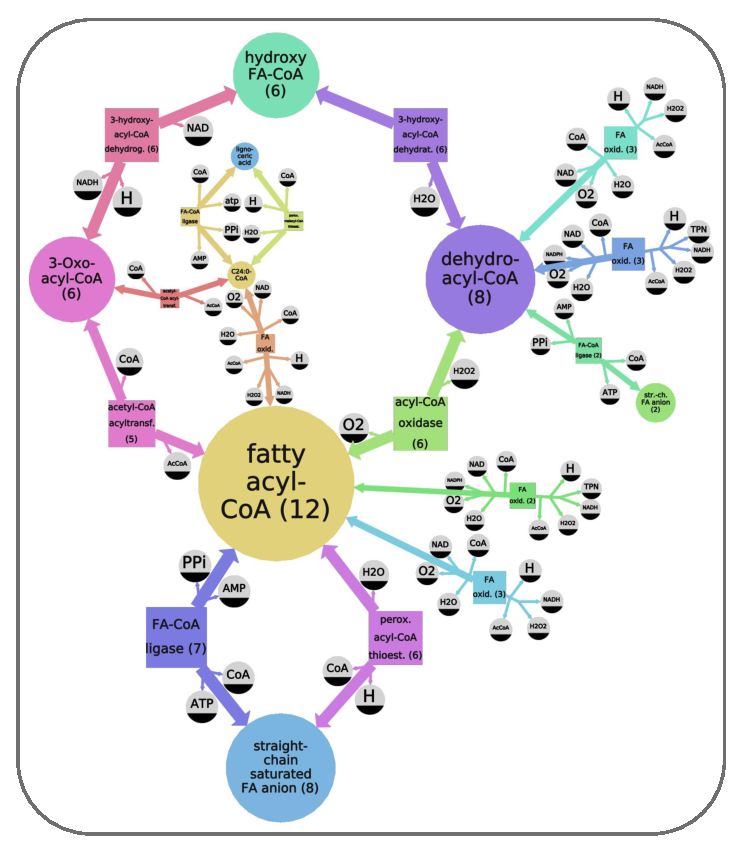
\includegraphics{../pics/Zhukova_Fig_2.eps}}
\vspace*{8pt}
\caption{\textbf{Peroxisome of the \textit{Y.~lypolitica} model (\emph{MODEL1111190000}).} Species are represented as circular nodes, and the reactions as squared ones, connected by edges to their reactants/products, according to SBGN notation~\citep{Moodie2011}. Ubiquitous species are of smaller size and coloured gray. Specific species are divided into six non-trivial equivalence classes, and coloured accordingly (violet, light-blue, yellow, green, light-green, magenta). The specific species that form trivial equivalence classes are all coloured red. Reactions are divided into fifteen non-trivial equivalence classes, also represented by different colours. Reactions that form trivial equivalence classes are all coloured blue.       
      The size of the model does not allow for readability of the species labels, thus we do not show them.}
\label{fig:bf}
\end{figure}

\begin{figure}[th]
\centerline{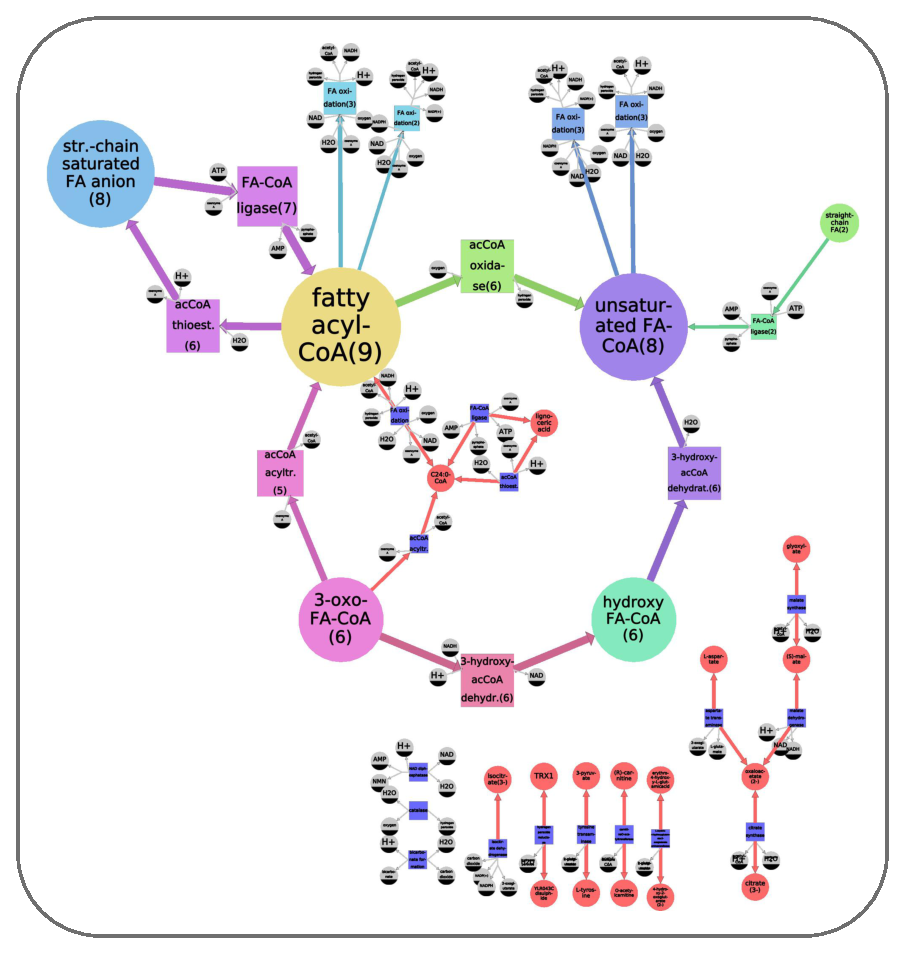
\includegraphics{../pics/Zhukova_Fig_3.eps}}
\vspace*{8pt}
\caption{\textbf{The generalization of the peroxisome of the \textit{Y.~lypolitica} model} (see figure~\ref{fig:bf}). The generalized model operates with quotient species and reactions. The number given in parenthesis and the size of each node indicates how many entities it generalizes.}
\label{fig:yali}
\end{figure}

\newpage
\section*{Discussions}

We have developed a method that provides a semantically zoomed-out view of a metabolic model, that keeps its essential structure but hides the details. 

We have implemented our method as a Python program, that is available for download from\\ \url{http://metamogen.gforge.inria.fr}. It takes an SBML model as an input, annotates its species with ChEBI terms (if the annotations are not present in the model) and generalizes it. It produces two SBML files, as an output. The first output file contains the generalized model. The second output file uses groups\citep{Hucka2012} extension of SBML, and contains the initial model plus the groups representing quotient species and reaction sets.

We have applied our method to genome-scale metabolic model of \emph{Y. lipolytica} and have shown that it helps finding gaps and peculiarities, as well as compresses the information stored in the model, which can be used for model visualisation and model comparison.

Currently the method depends on ChEBI ontology. It cannot generalize species that lack ChEBI annotations. The future work will include finding ways to overcome this limitation.

The method zooms out a model to the most general level of abstraction that is consisted with the model structure, i.e. does not violate the restrictions (1') and (2). It remains to be seen if there are intermediate levels of abstraction that can be useful for the model analysis. 

\bigskip

\section*{Acknowledgements}
  The authors would like to thank Dr. Romain Bourqui and Dr. Antoine Lambert of the LaBRI MABioVis team for advice on graph layout.
  
  AZ was supported by a CORDI-S doctoral fellowship from Inria.

\section*{Author Disclosure Statement}
No competing financial interests exist.

\newpage
 \bibliographystyle{zhukova-jcb}\bibliography{../db}


\section*{Additional Files}
  \subsection*{Additional file 1 --- The generalized SBML level 2 version 4 model of \textit{Yarrowia lipolytica} (derived from \emph{MODEL1111190000})}
    The model contains generalized reactions and species.
    
  \subsection*{Additional file 2 --- The SBML level 3 version 1 model of \textit{Yarrowia lipolytica} (derived from \emph{MODEL1111190000}) with groups extension representing equivalent species and reactions}
    The model contains all the elements (reactions, species, etc.) of the initial \emph{MODEL1111190000} model, and is enriched with groups representing species and reaction equivalence information.
    
  %  \subsection*{Additional file 3 --- Compartments of \textit{Yarrowia lipolytica} (\emph{MODEL1111190000}) model before and after generalization}
  %  A zip archive containing png pictures.
    

\end{document}  
